%\normalfont
\documentclass[10pt,conference,letterpaper]{IEEEtran}
\usepackage[pdftex]{graphicx}
\usepackage{graphicx}
\usepackage[table]{xcolor}
\usepackage{booktabs}
\usepackage{tabularx}
%\usepackage{balance}
\usepackage{makecell}
\usepackage{array}
\usepackage{cite}
\usepackage{hyperref} % for the url and hyperref
\usepackage{url}
\usepackage{float}
\usepackage{wrapfig}
\usepackage{amsmath}

\IEEEoverridecommandlockouts

\begin{document}

\bstctlcite{bstctl:etal}

\title{LLMMMM: Large Language Models Matrix-Matrix Multiplications Characterization on Open Silicon}

\author{\IEEEauthorblockN{Louis Ledoux\IEEEauthorrefmark{1}\IEEEauthorrefmark{2},
Marc Casas\IEEEauthorrefmark{1}\IEEEauthorrefmark{2}
}
\IEEEauthorblockA{\IEEEauthorrefmark{1}Barcelona Supercomputing Center, Barcelona, Spain}
\IEEEauthorblockA{\IEEEauthorrefmark{2}Universitat Polit\`ecnica de Catalunya, Barcelona, Spain}

E-mail: \{louis.ledoux,marc.casas\}@bsc.es\\

}

\maketitle

%ABSTRACT - Dis-comment the following lines to add an abstract
%\begin{abstract}
%You can add an abstract here
%\end{abstract}

\begin{keywords}
	Large Language Models (LLM), Transformers, Generative Pre-Trained (GPT), Matrix-Matrix Multiplications, Floating-Points, arithmetic, ASIC, Open-Source Silicon (OSS)
\end{keywords}

\vspace{-4mm}
%%%%%%%%%%%%%%%%%%%%%%%%%%%%%%%%%%%%%%%%%%%%%%%%%%%%%%%%%%%%%%%%%%%%%%%%%%%%%%%
%%% Introduction
%%%%%%%%%%%%%%%%%%%%%%%%%%%%%%%%%%%%%%%%%%%%%%%%%%%%%%%%%%%%%%%%%%%%%%%%%%%%%%%
\section{Extended Abstract}
%\subsection{Introduction}
%\label{sec:introduction}
%
%GPT transformers are usefol for ..
%
%However, they cost a lot Prior work show the cost of~\cite{luccioni2022estimating}
%
%Esentially MMM, wity hdatya movement of datum, the arithmetic weigts etc.. (describe the matrices, number of elements)
%
%Recent work focus on designing Specialized format and algorithm to reduce the cost (reducing bitwdith, MLX, tpu, bitnet, ternary, 40\% layer remove)
%
%We introduce a generator of ASIC kernels agnostic to the PDK of MMM units of emerging and small floating point formnats, we then evaluate such units.

\subsection{Introduction}
\label{sec:introduction}

GPT transformers are useful for various applications, offering significant advancements in natural language processing tasks.
However, their operational costs are substantial has shown in prior work which highlights the financial implications of deploying these models~\cite{luccioni2022estimating}.

Essentially, matrix-matrix multiplications (MMM), with their intensive data movement and manipulation of arithmetic weights, underscore the computational demands of these architectures.
Naturally, these observations are also found in recent efforts within the research community, which have concentrated on devising specialized formats and algorithms aimed at mitigating these costs.
These innovations include reducing bit-width exemplified by Machine Learning eXchange (MLX) formats (essentially small floats)~\cite{}, specialized hardware such as TPUs' systolic arrays~\cite{}, model pruning of up to 40\%~\cite{}, and more recently, ternary and binary LLMs (see BitNets~\cite{}).

We introduce a generator of ASIC kernels agnostic to the PDK of MMM units for emerging and small floating-point formats, followed by the evaluation of such units.
Concretely, our contributions include the automated generation of circuits for any floating-point format with automated pipelining, a systolic array architecture proposal—these two combined form the foundation of MMM units, a framework to automate the translation from high-level language (Python) to silicon for such matrices (SUF, SuperSet Framework~\cite{}), the generation of $7 \text{ arithmetic formats} \times 2 \text{ accumulator configurations} \times 4 \text{ PDKs} = 56$ chips, and their performance and efficiency evaluation, all provided as open source.

\subsection{Asynchronous and Parallel Compilation}
\label{sec:framework}
The need for fast generation of specialized circuits is mostly explained by the the known computer science laws being challegend (dennard, moore, the walls, dark silicon era).
A recent and emerging solution that allows to follow the pace is OpenSource EDA and its community~\cite{Openroad}.
We adopt this approach and build our own open source tool.
Figure~\ref{fig:suf} depicts this framework which enables the generation of many independant design entries from high level description in python to silicon GDS.

\begin{figure}[t]
\centering
	\vspace{-0.5cm}
	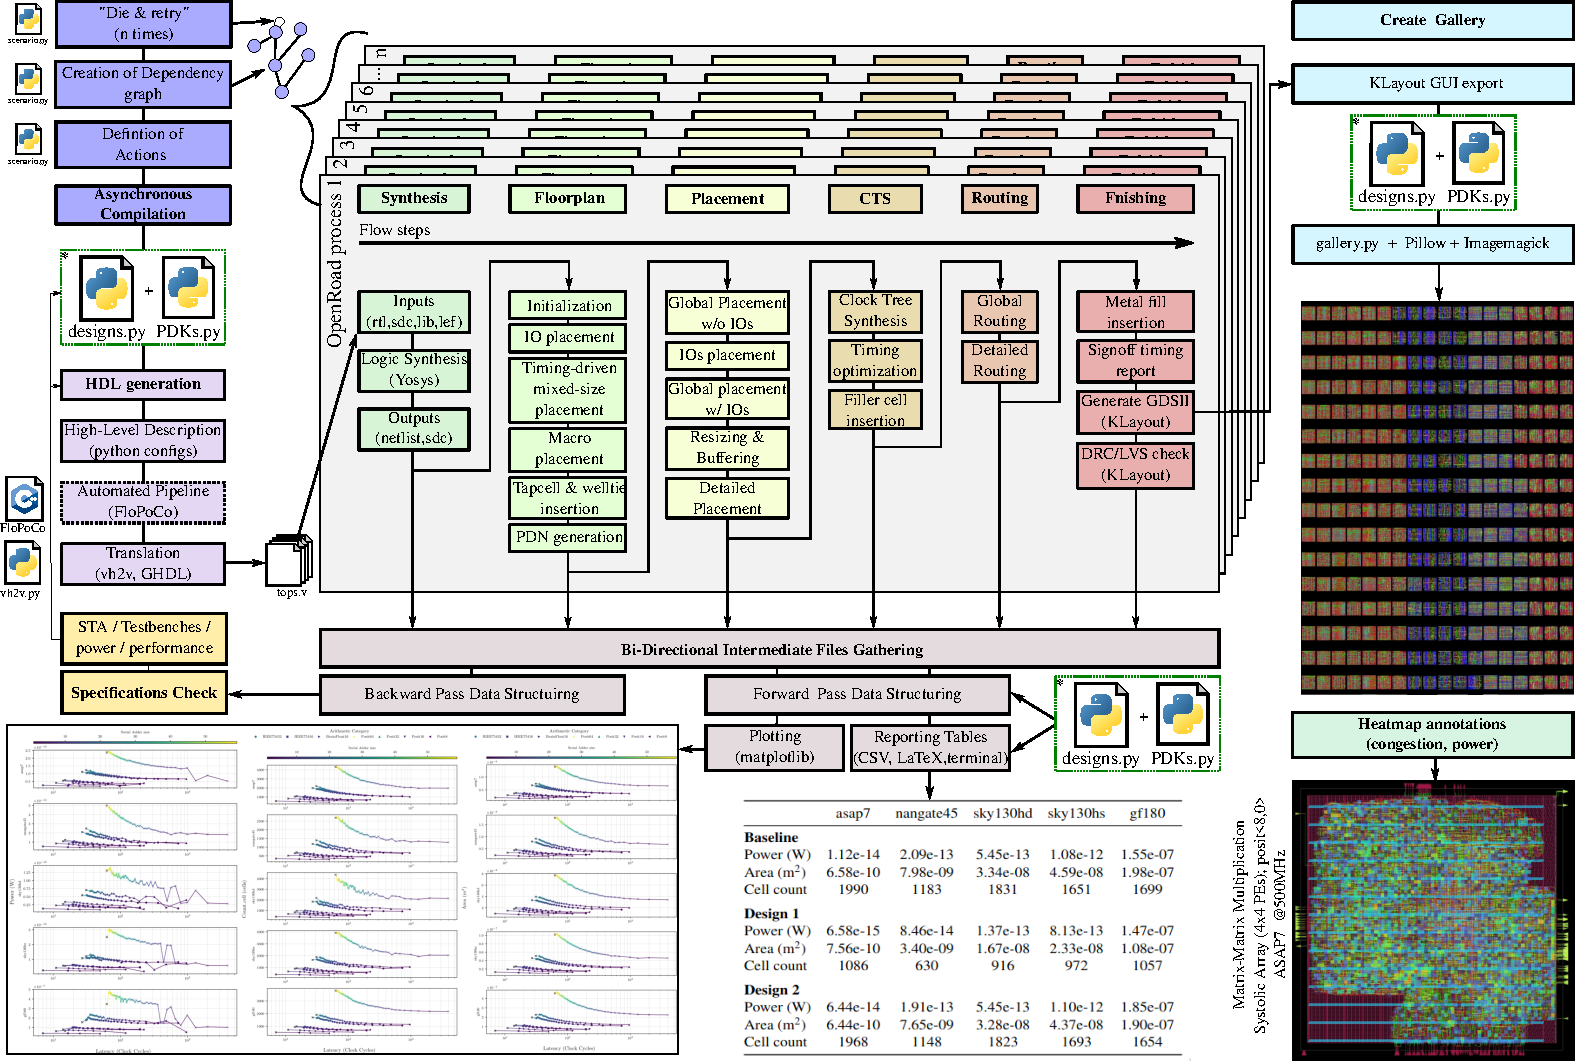
\includegraphics[width=\columnwidth]{./figures/SUF.pdf}
	\vspace{-0.5cm}
	\caption{Schematic Overview SUF: Centralized Management of Asynchronous OpenROAD Forks, Derived from Dependency Task Graphs. This illustration also encapsulates the extended capabilities ranging from Code Generation without manual RTL Writing to Advanced Plotting and Visualization Features.}
	\label{fig:suf}
\end{figure}

\begin{figure}[b]
\centering
	\vspace{-0.5cm}
	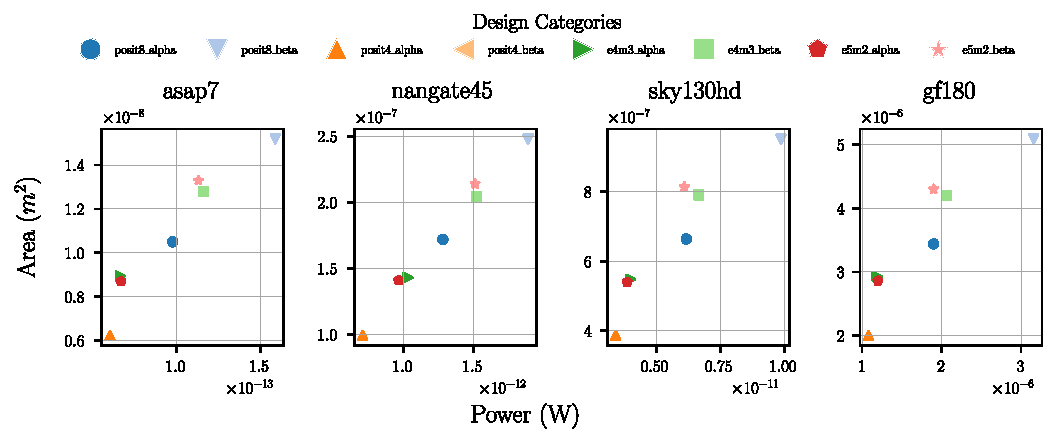
\includegraphics[width=\columnwidth]{./figures/power_vs_area_comparison.pdf}
	\vspace{-0.5cm}
	\caption{Area vs. Power}
	\label{fig:power_vs_area}
\end{figure}

\subsection{Functional and Performance Specifications}
\label{sec:specifications}
We define and assess four computational formats distinguished by their compactness and mathematical attributes (dynamic range).
These include Nvidia's e4m3 and e5m2, and the tapered formats, posit4 (es=0), and posit8(es=2)~\cite{}.
Another significant aspect of our work is the proposal of two variations of internal paths for each of these formats.
Internally, we execute the dot product as a fused operation (without rounding) in a fixed accumulator with varying boundaries (bit weights for lsb/msb/ovf).
These variations, named $\alpha$ and $\beta$, are configured as follows: $(\text{ovf}=2,\text{msb}=3,\text{lsb}=-2)$ for an aggregate of 8 bits, and $(\text{ovf}=5,\text{msb}=5,\text{lsb}=-5)$ for the 16-bit model.
The weights distribution of the embedding layers in the Llama-2-7b model~\cite{} dictates these boundaries.
%It is vital to evaluate the trade-offs in the accelerator segment robustly, considering the dynamic range of formats, precision, and sequentialism inherent in MMM algorithms.
All Systolic Arrays of this work are set to $8x8=64$ PEs, which ends the defintion of the \textit{Functional} specifications set.

% Performance properties
We complement this set with \textit{Performance} specifications that span four accross four PDKs, namely GF180, Sky130hd, nangate45, and ASAP7 which are all open (TBD).
Evaluation of several PDKs allow to verify scalability of designs without the use of manual scaling which are often (make it formal and scientific).

\subsection{Results}
The evaluation of 14 design entries, with posit 4 beta not working finished in two hours yielding a total of xx chips.
Figure~\ref{fig:power_vs_area} shows depicts power and area accross 5 process nodes.



\begin{figure}[t]
\centering
	\vspace{-0.5cm}
	\includegraphics[width=0.5\columnwidth]{./figures/SA_8x8_e4m3_rulers_congestion.png}
	\vspace{-0.5cm}
	\caption{e4m3 cogestion routed highlighted beta 8x8}
	\label{fig:focus on e4m3}
\end{figure}

\begin{figure}[t]
\centering
	\vspace{-0.5cm}
	\includegraphics[width=\columnwidth]{./figures/systolic_arrays.png}
	\vspace{-0.5cm}
	\caption{All generated arrays}
	\label{fig:all_arrays}
\end{figure}


\subsection{Conclusions}
\label{sec:conclusions}
Overall, by the mean of a custom open source framework, we are able to generate MMM units for several arithmetic specifciations and ttechnology nodes.
We show the performance metrics of 28 distinct chips that have been generated within an hour, which is possible thanks to open source EDA tools.

As a future perpectives, we need to correlate the performance metrics measured with accuracy metrics in order to find the best entry in the vast accuracy/energy efficiency design space exploration.
In light of these promising results, we ecnourage researchers to interact with our tool.

\subsection{Biography}
\label{sec:biography}

\begin{wrapfigure}{l}{0.2\textwidth} % "l" for left and "0.25\textwidth" for the width of the wrap figure area
\centering
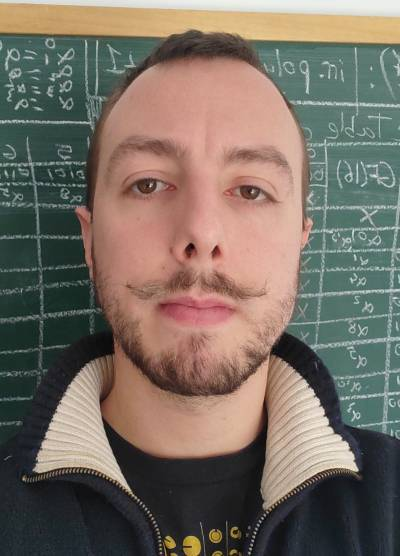
\includegraphics[width=0.18\textwidth]{./figures/louis2.jpg}
\end{wrapfigure}
Louis Ledoux, originating from a comprehensive computer science background in Rennes (Bretagne, France), has transitioned towards a hardware focus. His journey began with a Bachelor's degree, followed by a Master's in Computer Science, culminating in a one-year internship in 2017, where he explored FPGA virtualization in the cloud. Since 2018, Louis has been engaged in a PhD in computer arithmetic at the Universitat Polit\`ecnica de Catalunya and the Barcelona Supercomputing Center, in Barcelona, Spain. His main focus are hardware implementations to address numerical requirements sparsity in HPC workloads. Beyond academia, Louis contributes to the open hardware community, participating in efabless/skywater/Google tapeouts.

%\begin{figure}[H]
%\begin{minipage}[b]{0.1\linewidth}
%\centering
%	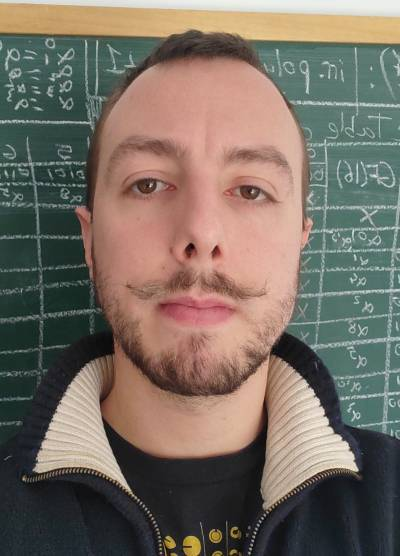
\includegraphics[width=\textwidth]{./figures/louis2.jpg}
%\end{minipage}
%\hspace{0.5cm}
%\begin{minipage}[b]{0.85\linewidth}
%\centering
%Louis Ledoux, originating from a comprehensive computer science background in Rennes (Bretagne, France), has transitioned towards a hardware focus.
%His journey began with a Bachelor's degree, followed by a Master's in Computer Science, culminating in a one-year internship in 2017, where he explored FPGA virtualization in the cloud.
%Since 2018, Louis has been engaged in a PhD in computer arithmetic at the Universitat Polit\`ecnica de Catalunya and Barcelona Supercomputing Center, in Barcelona, Spain.
%His main focus are hardware implementations to address numerical requirements sparsity in HPC workloads.
%Beyond academia, Louis contributes to the open hardware community, participating in efabless/skywater/Google tapeouts.
%\end{minipage}
%\end{figure}

\section{Acknowledgment}
\label{sec:acknowledgment}
Marc Casas has been partially supported by the Grant RYC-2017-23269 funded by MCIN/AEI/10.13039/501100011033 and by ESF Investing in your future. This research was supported by grant PID2019-107255GB-C21 funded by MCIN/AEI/ 10.13039/501100011033. Els autors agraeixen el suport del Departament de Recerca i Universitats de la Generalitat de Catalunya al Grup de Recerca "Performance understanding, analysis, and simulation/emulation of novel architectures" (Codi: 2021 SGR 00865).


\IEEEpeerreviewmaketitle

\vspace{-2mm}


\vspace{-2mm}

%%%%%%%%% -- BIB STYLE AND FILE -- %%%%%%%%
%\balance
\bibliographystyle{IEEEtran}
%\bibliography{IEEEabrv,paper}

\bibliography{references.bib}
\vspace{-7mm}
%%%%%%%%%%%%%%%%%%%%%%%%%%%%%%%%%%%%

\end{document}
